% !Mode:: "TeX:UTF-8"
\chapter{可见光多波段OFDM系统的信道估计}
\section{引言}
所谓信道估计,就是在接收端估计出信道状态信息(Channel State Information,CSI),为下一步地解调做准备,也是自适应传输技术的基础。无线通信一个重要的特征就是发射端到接收端之间的路径比较复杂,不像有线通信那样是固定且可预知的,所以信道估计技术在无线通信领域格外重要,特别是在OFDM 等需要相干检测的系统中。本章将着重介绍信道估计技术,首先介绍传统射频通信中OFDM 系统的信道估计方法,然后具体到可见光通信系统中的信道估计问题,再将结合实际系统设计,讨论信道的非线性问题,最后将研究多色可见光通信系统中各波段之间串扰的估计。
\section{OFDM信道估计常用方法}
信道估计总体可以分为两大类,盲信道估计和基于导频的信道估计。盲信道不需要额外的导频或者训练序列,因此频率利用率高;但是它的缺点是计算量大、算法复杂,而且精度低、收敛速度缓慢,难以用于移动通信环境
\cite{石钧2012ofdm}。基于导频的信道估计原理是在发射端插入专门用于信道估计的导频或者训练序列,并且这些序列对于接收端也是已知的,接收端根据接收到的经过了信道后的导频序列与原导频序列之间的关系,估计出信道冲击响应(Channel Impulse Response,CIR)。这类信道估计方法因为要插入导频序列会稍微降低整个系统的传输速率,但是其估计实现复杂度低、估计精度高,在实际工程中大都采用这种方法。本节也主要讨论基于导频的信道估计算法。
\begin{figure}[htbp]
    \centering
    \subfloat[块状导频放置方式]{
        \label{fig:BlockTypePilot}
        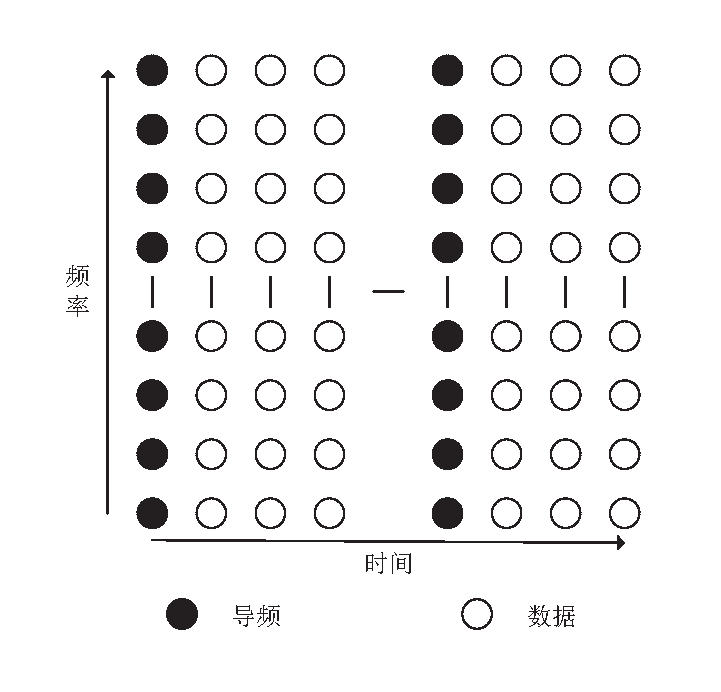
\includegraphics[width = 0.5\textwidth]{figures/chapter-3/BlockTypePilot.eps}
    }
    \subfloat[梳状导频放置方式]{
    	\label{fig:CombTypePilot}
        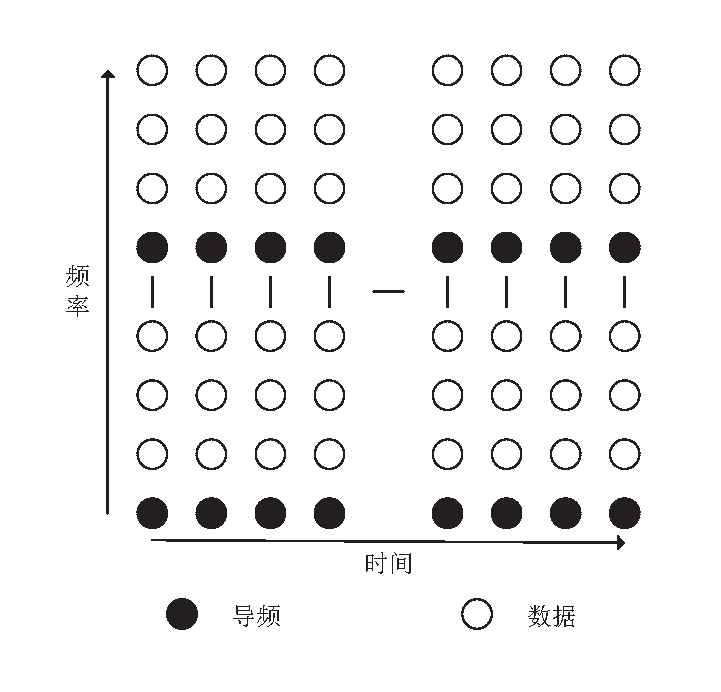
\includegraphics[width = 0.5\textwidth]{figures/chapter-3/CombTypePilot.eps}
    }
    \caption{导频放置方式}
    \label{fig:PilotAllocation}
\end{figure}
对于基于导频的信道估计而言,研究人员对其导频放置方式也进行了深入的研究,如\autoref{fig:PilotAllocation} 所示,常见的有块状和梳状两种放置方式。

块状导频放置方式见图\ref{fig:BlockTypePilot},它的导频序列连续放置在一个OFDM符号上,但是在时间上不是连续的,也就是说要隔若干个OFDM符号才放置一个导频序列。在工程实现中,更常见的一种情况是导频序列即用于信道估计,又用于同步,这样一般是一帧放置一个导频符号。块状导频放置方式的优点是结构简单,计算复杂度低,但是因为要隔一段时间才估计一次信道,所以块状导频放置方式一般用于信道时变比较缓慢的信道。

梳状导频放置方式如图\ref{fig:CombTypePilot}所示,在每个OFDM符号上,它只选择在特定的子载波上放置导频序列,而其他子载波上放置数据符号,并且每个OFDM 符号的结构都是如此。它的工作原理是先估计出放置了导频的子载波处的信道响应,然后根据这些信道响应通过插值的方式得到那些放置了数据符号的子载波处的信道响应。它的优点是每个符号都会估计信道,能够应对快速时变的信道,但是它要使用插值计算,所以复杂度比较高,并且估计准确度也较低。

为了说明这两种基于导频信道估计的工作原理,我们先建立OFDM 数字处理模型,并且假设循环前缀的长度大于最大多径时延,则根据我们在第二章中线性信道模型可得:
\begin{equation}
\bf y=h\otimes x+z
\label{equ:time-domain signal}
\end{equation}
其中$\otimes$表示线性卷积运算,$\textbf x$为发射信号向量,$\textbf y$ 为接收信号向量,$\textbf x$为噪声信号向量,并且假设发射信号向量$\textbf x$ 的长度为$N$。根据同步信号,除掉接收信号向量$\textbf y$中的循环前缀,然后再取长度等于$N$的序列$\textbf y_c$,$\textbf y_c$即为$\textbf x$ 与$\textbf h$ 的长度为$N$的圆周卷积结果,根据DFT 的圆周卷积特性有:
\begin{equation}
\bf Y=XH+Z
\label{equ:chapter-3-3}
\end{equation}
其中$\textbf X$表示频域发射信号,$\textbf Y$表示频域接收信号,$\textbf Z$表示频域高斯噪声,$\textbf F$表示离散傅里叶变换矩阵,它们的具体表达式如下:
\begin{equation}
\begin{aligned}
&\textbf X=diag(DFT(\textbf x))==diag([ X(0), X(1),..., X(N-1)]^T)\\
&\textbf Y=DFT(\textbf y_c) =[ Y(0), Y(1),..., Y(N-1)]^{T} \\
&\textbf Z=DFT(\textbf z) =[ Z(0), Z(1),..., Z(N-1)]^{T} \\
&\textbf H=DFT(\textbf h) =[ H(0), H(1),..., H(N-1)]^{T} \\
\end{aligned}
\end{equation}
\subsection{基于块状导频的信道估计}
块状导频放置方式将导频序列放在连续的一个OFDM符号子载波上,所以最直接的方式就是利用这些导频序列来估计信道冲激响应,即等效为在式
\ref{equ:chapter-3-3}中已知了频域发射信号$\textbf X$,估计信道频域响应$\textbf H$,常见的估计方法有最小二乘法准则(Least Square,LS)、最小均方误差估计准则(minimum mean square error,MMSE)、线性最小均方误差准则(linear minimum mean square error,LMMSE )及基于SVD分解的MMSE算法等。
\subsubsection{LS估计算法}
基于LS准则的的估计算法目标是使得接收信号与通过该模型恢复出来的信号之间的距离最小,假设LS算法的结果是${\hat{\textbf H}}_{LS}$,则其目标函数为:
\begin{equation}
arg\ \underset {{\hat{\textbf H}}_{LS}}{min}\ \textbf {L}({\hat{\textbf H}}_{LS})
=arg\ \underset {{\hat{\textbf H}}_{LS}}{min}\left \{  {\left |\textbf Y- \textbf X{\hat{\textbf H}}_{LS} \right|}^2\right \}
\label{equ:chapter-3-4}
\end{equation}
将上面的目标函数展开可得:
\begin{equation}
\textbf {L}({\hat{\textbf H}}_{LS}) = \sum_{i=0}^{N-1} {|Y(i)-X(i)\hat{H}_{LS}(i)|}^2
\end{equation}
所以式\ref{equ:chapter-3-4}取得最小值时必有:
\begin{equation}
\hat{H}_{LS}(i) = \frac{Y(i)}{X(i)} \ \ (i=0,1,2,...,N-1)
\end{equation}
也可以写为向量形式为:
\begin{equation}
{\hat{\textbf H}}_{LS} =\bf X^{-1}Y
\label{equ:Least Square channel Estimation}
\end{equation}
从上面最后的结果看出最小二乘估计算法计算复杂度非常简单,只需要两次傅里叶变换和$N$次复数除法即可,但是它没有考虑噪声的影响,在信噪比不高的情况下,估计精度不高。
\subsubsection{MMSE估计算法}
可以使用信道冲激响应和噪声的统计特性来提高估计精度,MMSE 算法假设信道冲激响应$\textbf H$与噪声$\textbf Z$ 是相互独立的,同时利用信道和噪声的二阶统计量来帮助提高信道估计的准确度,可以利用二阶统计量提高精度的原因是二阶统计量是慢时变的。
MMSE估计算法的目标是使得信道估计值与真实值之间的误差最小:
\begin{equation}
arg\ \underset {{\hat{\textbf H}_{MMSE}}}{min}\ {\textbf M} ({\hat{\textbf H}_{MMSE}})=arg\ \underset {{\hat{\textbf H}_{MMSE}}}{min}\left \{  {\left |{\textbf H_{R}}- {\hat{\textbf H}_{MMSE}} \right|}^2\right\}
\end{equation}
上式中$\textbf H_R$表示真实信道的频域冲激响应,MMSE 的解为\cite{Kay1993FSS}:
\begin{equation}
\hat{\textbf H}_{MMSE}= \textbf R_{HY}\textbf R_{YY}^{-1}\textbf Y
\label{equ:MMSE1}
\end{equation}
其中$\textbf R_{HY}$表示信道频域响应$\textbf H$与接收信号$\textbf Y$之间的互协方差矩阵,$\textbf R_{YY}$表示$\textbf Y$的自相关矩阵,具体表达式如下:
\begin{equation}
\begin{aligned}
\textbf R_{HY}&=E(\textbf H{\textbf Y}^H)={\textbf R}_{HH}{\textbf X}^H \\
\textbf R_{YY} &= E({\textbf Y}{\textbf Y}^H)={\textbf X}{\textbf R}_{HH}{\textbf X}^H + \sigma_n^2{\textbf I}_N
\end{aligned}
\label{equ:MMSE2}
\end{equation}
上式中$\textbf R_{HH}=E(\textbf H {\textbf H}^H)$表示信道冲激响应的自相关矩阵,$\sigma_n^2$为加性高斯白噪声的方差,$\textbf I_N$为$N\times N$的单位矩阵。结合式\ref{equ:Least Square channel Estimation}、\ref{equ:MMSE1} 及\ref{equ:MMSE2},MMSE信道估计的结果可以用LS信道估计的结果来表示:
\begin{equation}
\hat{\textbf H}_{MMSE}= \textbf R_{HH}(\textbf R_{HH}+\sigma_n^2(\textbf X \textbf X^H)^{-1})^{-1}{\hat{\textbf H}_{LS}}
\label{equ:MMSE3}
\end{equation}
这里我们可以看出MMSE估计算法的计算复杂度比较高,需要矩阵的相关及求逆运算,并且它的复杂度会随着子载波数目增加而成指数上升。
\subsubsection{LMMSE估计算法}
LMMSE是对MMSE的简化,使用$E[(\textbf X \textbf X_H)^{-1}]$ 来代替式\ref{equ:MMSE3}中的$(\textbf X \textbf X_H)^{-1}$\cite{付可2015lte},并且考虑到发射信号$\textbf X$各子载波上的符号是随机等概地取自调制符号星座点的,所以有:
\begin{equation}
E[(\textbf X \textbf X^H)^{-1}]=E[|1/x_k|^2]\textbf I_N
\end{equation}
再结合平均信噪比的定义$SNR=E[|x_k|^2]/{\sigma_n^2}$ 将其代入式\ref{equ:MMSE3} 可得:
\begin{equation}
\hat{\textbf H}_{LMMSE}=\textbf R_{HH}(\textbf R_{HH}+\frac{\beta}{SNR}\textbf I_N)^{-1}\hat{\textbf H}_{LS}
\label{equ:LMMSE1}
\end{equation}
其中$\beta$是与调制星座图相关的常量\cite{张乃元2010lte},从式\ref{equ:LMMSE1}中可以看出,LMMSE算法的复杂度相对于MMSE已经降低了不少,但是总的来说还是需要计算$\textbf R_{HH}$和矩阵求逆,复杂度还是偏高的,但其保留了MMSE的核心思想,相较于MMSE性能损失不大。
\subsubsection{基于SVD分解的MMSE估计算法}
由前面的分析可知,LMMSE虽然对MMSE算法进行了简化,但是还是需要计算自相关矩阵$\textbf R_{HH}$和矩阵求逆,为了进一步简化运算,可以对式\ref{equ:LMMSE1}中系统$\textbf R_{HH}$ 这个$N\times N$矩阵进行奇异值分解:
\begin{equation}
\textbf R_{HH} = U \Lambda U^H
\label{equ:SVD1}
\end{equation}
上式中$U$为酉矩阵,$\Lambda$为对角阵,其对角线上的元素为矩阵$\textbf R_{HH}$ 的特征值,并且从大到小排列($\lambda_1\geq\lambda_2\geq\cdots\geq\lambda_N$), 式\ref{equ:SVD1} 代入式\ref{equ:LMMSE1} 得:
\begin{equation}
\begin{aligned}
\hat{\textbf H}_{LMMSE}&=U\left[\Lambda\left(\Lambda+\frac{\beta}{SNR}\textbf I_N\right)^{-1}\right]U^H\hat{\textbf H}_{LS} \\
&=U\left[diag\left(\frac{\lambda_1}{\lambda_1+\frac{\beta}{SNR}},\frac{\lambda_2}{\lambda_2+\frac{\beta}{SNR}},\cdots,\frac{\lambda_N}{\lambda_N+\frac{\beta}{SNR}}\right)\right]U^H\hat{\textbf H}_{LS}
\end{aligned}
\end{equation}
为了进一步简化运算,可以只取$\textbf R_{HH}$前$M$个比较大的特征值$\lambda_1,\lambda_2,\cdots,\lambda_M$,将最后N-M 个较小的特征值为零,记为:
\begin{equation}
\hat{\textbf H}_{SVD}=U \begin{bmatrix}\Delta_M & 0 \\ 0 & 0 \end{bmatrix} U^H \hat{\textbf H}_{LS}
\end{equation}
其中$\Delta_M = diag\left(\frac{\lambda_1}{\lambda_1+\frac{\beta}{SNR}},\frac{\lambda_2}{\lambda_2+\frac{\beta}{SNR}},\cdots,\frac{\lambda_M}{\lambda_M+\frac{\beta}{SNR}}\right)$,SVD分解算法将原来MMSE算法中的矩阵相关和求逆运算变成了矩阵的SVD分解,并且通过去掉较小的特征值来进行降低,进一步降低了复杂度。
\subsection{基于梳状导频的信道估计}
梳状导频放置方式如图\ref{fig:CombTypePilot}所示,在每个OFDM符号上只在特定的位置放置了导频训练序列,而其他的子载波都是放置数据的。它的估计方法是首先使用上节中LS、MMSE、LMMSE或者SVD分解方法估计出放置了导频训练序列处的信道冲激响应,然后再用插值法得到其他放置数据位置的信道冲激响应值。

假设在梳状导频放置方式中有M个子载波放置了导频序列,并且从第一个子载波处开始放置,则他们放置的位置为$k_0,k_1,\cdots,k_{M-1}$,其中$k_i=iD_f, i=0,1,\cdots,M-1$,$D_f=N/M$为导频放置间隔子载波数。此模型下发射数据$\textbf X=diag(X(0),X(1),\cdots,X(N-1))$ 可表示为:
\begin{equation}
X(k)=
\begin{cases}
P_i, \ k=iD_f \\
data, \ k=iD_f+d, d=1,2,\cdots,D_f-1
\end{cases}
\end{equation}
其中$P_m$表示导频序列,data表示发送数据,我们称放置了导频序列的子载波为导频子载波,而称放置了信息数据的子载波为数据子载波。则可以得到导频子载波的信道LS 估计值为:
\begin{equation}
\hat{H}_{LS}(k_i) = \frac{Y(k_i)}{P_i}, i=0,1,\cdots,M-1
\label{equ:Comb1}
\end{equation}
其中$Y(k),k=0,1,\cdots,N-1$为接收信息序列。为了提供信道冲激响应的估计准确度,我们也可以使用MMSE、LMMSE 或者SVD估计法,如LMMSE估计的结果为:
\begin{equation}
\hat{\tilde{\textbf H}}_{LMMSE}=\textbf R_{\tilde{H}\tilde{H}}(\textbf R_{\tilde{H}\tilde{H}}+\frac{\beta}{SNR}\textbf I_M)^{-1}\hat{\tilde{\textbf H}}_{LS}
\end{equation}
其中$\hat{\tilde{\textbf H}}_{LS}=[\hat{H}_{LS}(k_0),\hat{H}_{LS}(k_1),\cdots,\hat{H}_{LS}(k_{M-1})]^T$ 为式\ref{equ:Comb1}中得到的LS估计值,$\textbf R_{\tilde{H}\tilde{H}}=E(\tilde{H}\tilde{H})$为导频子载波频域信道冲激响应的自相关矩阵。

通过块状导频放置方式的LS、MMSE、LMMSE或者SVD分解估计法我们可以得到梳状导频放置方式中导频子载波的信道冲激响应,下面要通过插值来得到放置信息数据处的信道估计,常见的插值方法有一阶线性插值、二阶多项式插值及变换域插值等。
\subsubsection{一阶线性插值}
一阶线性插值就是利用相邻的两个导频子载波的信道冲激响应来计算他们之间的数据子载波的信道信息,对于任意一个位于第$m$ 个与第$m+1$个导频子载波之间数据子载波$k, mD_f<k<(m+1)D_f$,我们可以得到他的线性插值估计值为\cite{sandell1996comparative}:
\begin{equation}
\begin{aligned}
\hat{H}(k)&=\hat{H}(mD_f+d) \\
&=(\hat{H}(k_{m+1}-\hat{H}(k_m))\frac{d}{D_f}+\hat{H}(k_m)
\end{aligned}
\end{equation}
其中$m=0,1,\cdots,M-2$,$d=0,1,\cdots,D_f-1$。从上式中可以看到,在这个模型中最后一个子载波不是导频子载波,所以最后的$D_f-1$个数据子载波只能用最后两个导频子载波来估计,其表达式为:
\begin{equation}
\begin{aligned}
\hat{H}(k) &= \hat{H}((M-1)D_f+d) \\
&= (\hat{H}(k_{M-1})-\hat{H}(k_{M-2}))\frac{d}{D_f}+\hat{H}(k_{M-1})
\end{aligned}
\end{equation}
\subsubsection{二阶多项式插值}
一般而言,进行插值运算时,结果准确度会随着阶数的增加而增加\cite{garcia2000pilot},但是插值阶数越高,也就意味中计算复杂度越高,所以为了寻求准确度与复杂度之间的均衡,在工程中常用的插值方式还是一阶插值和二阶插值,二阶插值的表达式为:
\begin{equation}
\begin{aligned}
\hat{H}(k) &= \hat{H}(mD_f+d) \\
&=c_{-1}\hat{H}(k_{m-1})+c_0\hat{H}(k_m)+c_1\hat{H}(k_{m+1})
\end{aligned}
\end{equation}
其中$m=0,1,\cdots,M-3$,$d=0,1,\cdots,D_f-1$,$c_{-1}=\alpha(\alpha-1)/2$,
$c_0=-(\alpha-1)(\alpha+1)$,$c_1=\alpha(\alpha+1)/2$,$\alpha=d/D_f$。二阶多项式插值也存在最后的$2(D_f-1)$的数据子载波不适应上面的公式的问题,不过可以使用一阶插值来处理最后的这些子载波。
\subsubsection{变换域插值}
文献\onlinecite{zhao1997novel}中提出了一种基于FFT/IFFT变换的高精度插值方法。这种插值方法首先也是得到各导频子载波上的信道冲激响应估计值$\hat{H}(k_m)$,再进行M点FFT变换,将其变换到变换域:
\begin{equation}
Q_M(q)=\sum_{m=0}^{M-1}\hat{H}(k_m)e^{\frac{-j2\pi mq}{M}},\ q=0,1,\cdots,M-1
\end{equation}
然后在变换域进行补零,将整个序列长度由$M$点扩充为$N$ 点,补零的公式为:
\begin{equation}
Q_N(q)=
\begin{aligned}
\begin{cases}
Q_M(q), &0\leq q \leq P_c \\
0, &P_c < q < N-P_c \\
Q_M(q-N+M),&N-P_c \leq  q \leq N-1
\end{cases}
\end{aligned}
\end{equation}
其中$P_c$称为”截止频率“,可以将上式中补零的过程看出了个带阻滤波器,而$P_c$就决定了这个滤波器的带阻位置,$P_c$的选择要使得通带内的信道能量占总能量的90\% 到95\%,即保证\ref{equ:Tranform1}中$0.90\leq R \leq 0.95$。
\begin{equation}
R=\frac{\sum_{p=0}^{P_c}|\bar{Q}_M(p)|^2+\sum_{p=M-P_c}^{M-1}|\bar{Q}_M(p)|^2}{\sum_{p=0}^{M-1}|\bar{Q}_M(p)|^2}
\label{equ:Tranform1}
\end{equation}
上式中$\bar{Q}_M(p)$表示$Q_M(p)$的平均值。得到扩展后的变换域序列$\textbf Q_N$之后,可以用$N$点IFFT变换得到插值结果:
\begin{equation}
\hat{H}(k) = a\cdot \sum_{q=0}^{N-1}Q_N(q)e^{\frac{j2\pi qk}{N}}, \quad 0\leq k \leq N-1
\end{equation}
式中$a$的作用是均衡M点FFT变换与N点IFFT变换之间的系数变化。
\section{可见光通信中的信道估计}
\label{section:Channel_Estimation}
从上节的分析中可以看到基于导频的信道估计中导频子载波的放置有两种方式,一种是块状放置方式,另一种是梳状放置方式。梳状放置方式计算复杂度比较高,但是能够适应快速时变的通信环境,而块状放置方式结构简单,它适应于准静态的信道估计。室内可见光通信信道正是一种准静态信道,所以本课题主要研究基于块状放置的导频信道估计方法。
\subsection{可见光通信系统帧结构}
为了讨论实际系统中的信道估计,首先有必要介绍下可见光通信系统的OFDM帧结构及符号结构。如图\ref{fig:FrameStructure} 中所示是一个典型的DCO-OFDM 帧结构示意图,一个OFDM 帧由一个精心设计的导频符号开始,后面跟着$N$个数据符号,而在每个OFDM数据符号中,在N个可用子载波中,最低频的m个和最高频的n 个子载波被设置为虚拟子载波,即在这些子载波上置零而不放置任何数据,在高频设置虚拟子载波很容易理解,从第二章的分析中可以知道室内可见光信道时一个低通的信道,意味着高频子载波的信噪比可能不够,故不能传输数据,而在低频也要设置虚拟子载波是因为在接收端有个去掉DCO-OFDM偏置的隔直电路,其实就是一个高通滤波器,但是这个滤波器不是理想的,会对低频的几个子载波造成影响,所以也要将其设置为虚拟子载波;最后的N 个子载波是保证IFFT 结果为实数加的共轭对称子载波。在系统设计中,为了提高系统的实际传输速率,减少额外开销,选择的导频序列不但要用于信道估计,还要起到定时同步的作用。Zadoff-Chu (ZC)序列就是一种能够同时满足这两个条件的序列,下面先简要介绍下ZC序列。
\begin{figure}[htbp]
    \centering
    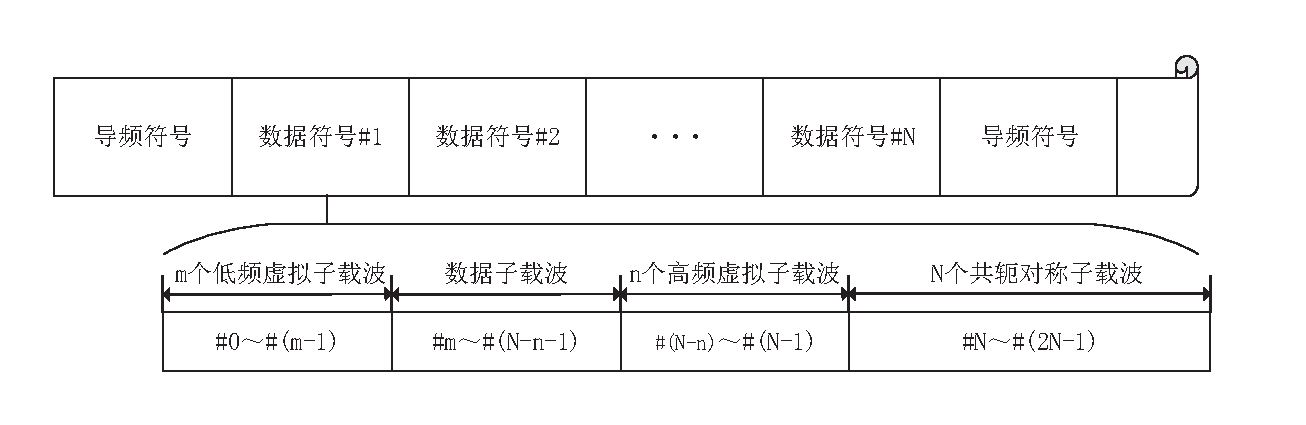
\includegraphics[width=0.8\textwidth]{figures/chapter-3/FrameStructure.eps}
    \caption{可见光通信系统帧结构}
    \label{fig:FrameStructure}
\end{figure}

ZC序列最早由Zadoff、Chu等人提出,具有非常好的自相关性和很低的互相关性的定义如下:
\begin{equation}
ZC(k)=
\begin{aligned}
\begin{cases}
e^{-\frac{2\pi r}{N}(k^2/2+qk)}, &N\text{为偶数}\\
e^{-\frac{2\pi r}{N}(k(k+1)/2+qk)}, &N\text{为奇数}
\end{cases}
\end{aligned}
\end{equation}
其中$k=0,1,\cdots,N-1$,$q$为任意的整数,$r$称为ZC序列的根指数,取值为小于$N$的正数据,并且要满足与长度$N$互素。
\begin{figure}[htbp]
    \centering
    \subfloat[频域幅度]{
        \label{fig:ZC_frequency}
        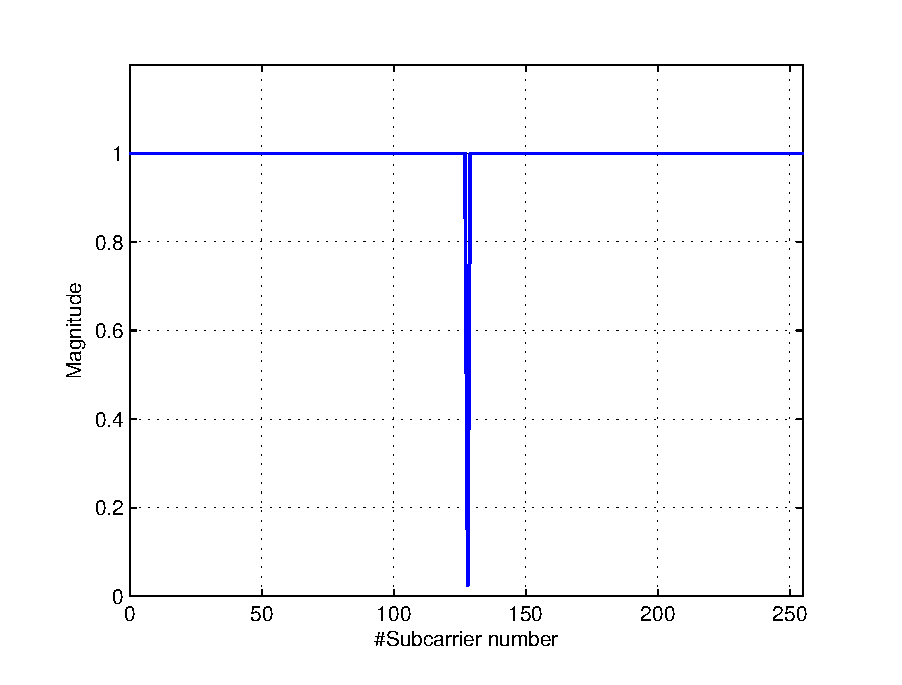
\includegraphics[width=0.5\textwidth]{figures/chapter-3/ZC_frequency.eps}
    }
    \subfloat[时域波形]{
        \label{fig:LZC_wavelengthShift}
        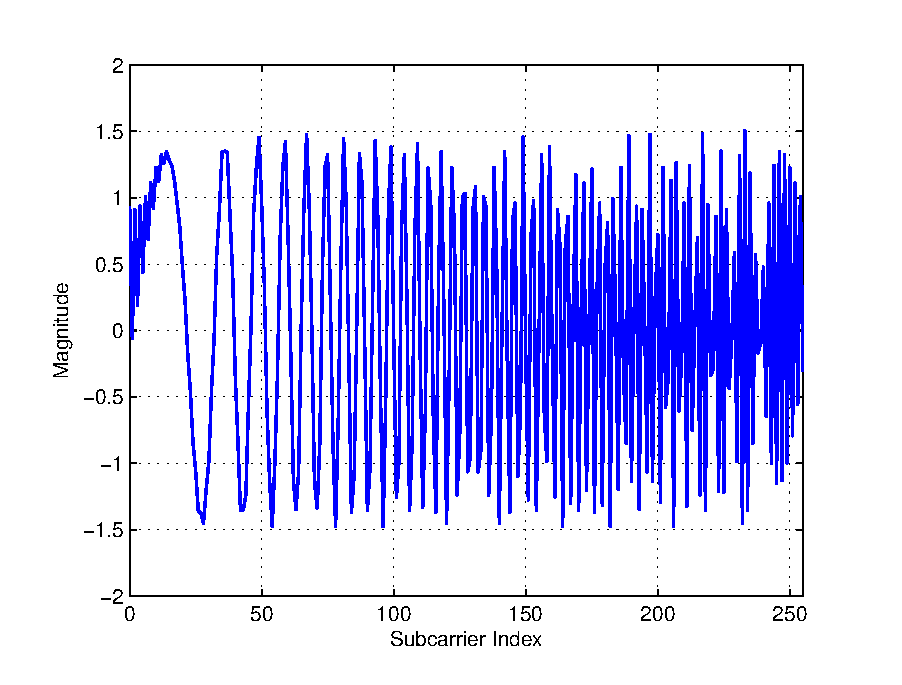
\includegraphics[width=0.5\textwidth]{figures/chapter-3/ZC_time.eps}
    }
    \caption{用于DCO-OFDM中ZC序列时频域波形}
    \label{fig:ZC_frequency_time}
\end{figure}
如图\ref{fig:ZC_frequency_time}所示为DCO-OFDM使用的ZC序列的示意图,该波形是由$N=128,q=0,r=1$的ZC序列加上128个共轭对称子载波形成的,在图\ref{fig:ZC_frequency}中,除了128号子载波处(放置0号子载波的虚部,故为零)之外,其他子载波的幅度都为1;时域波形为实数,并且其PAPR比较低,这个特性也可以减少信道估计中非线性的干扰。
\subsection{可见光信道仿真分析}
可以通过仿真的方法研究各种信道估计算法的性能,为了贴近实际的系统工作环境,仿真的信道取自\ref{subsection:Channel} 节中的实测可见光通信信道时域冲激响应,并且去掉其时延大,能量小的径,只留下能量其中的20径,并进行了能量归一化,其时域频域冲激响应如下图所示:
\begin{figure}[htbp]
    \centering
    \subfloat[时域冲激响应]{
        \label{fig:Sim_Channel_time}
        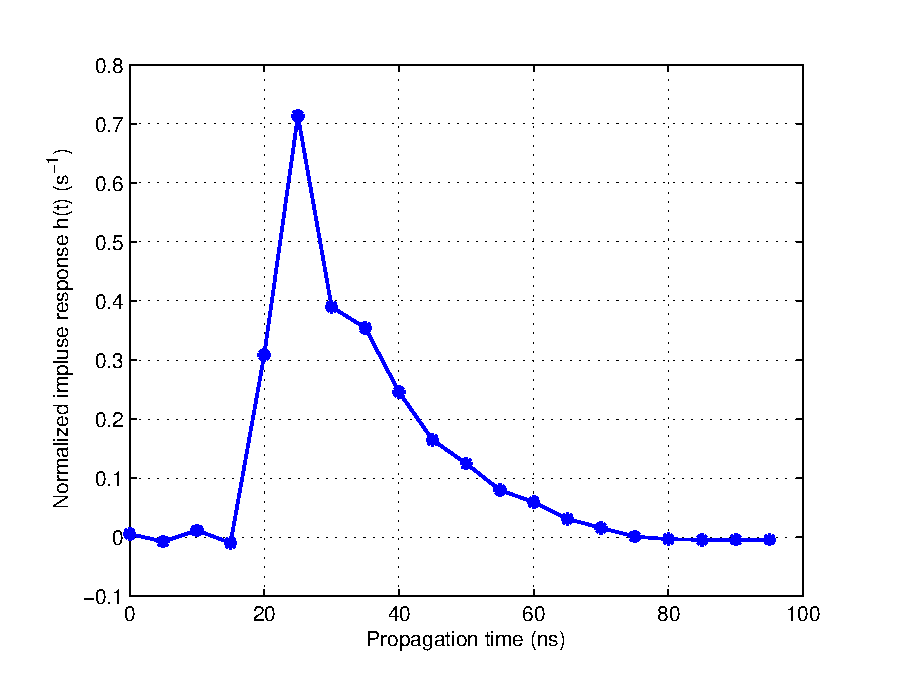
\includegraphics[width=0.5\textwidth]{figures/chapter-3/Sim_Channel_time.eps}
    }
    \subfloat[频域冲激响应]{
        \label{fig:Sim_Channel_frequency}
        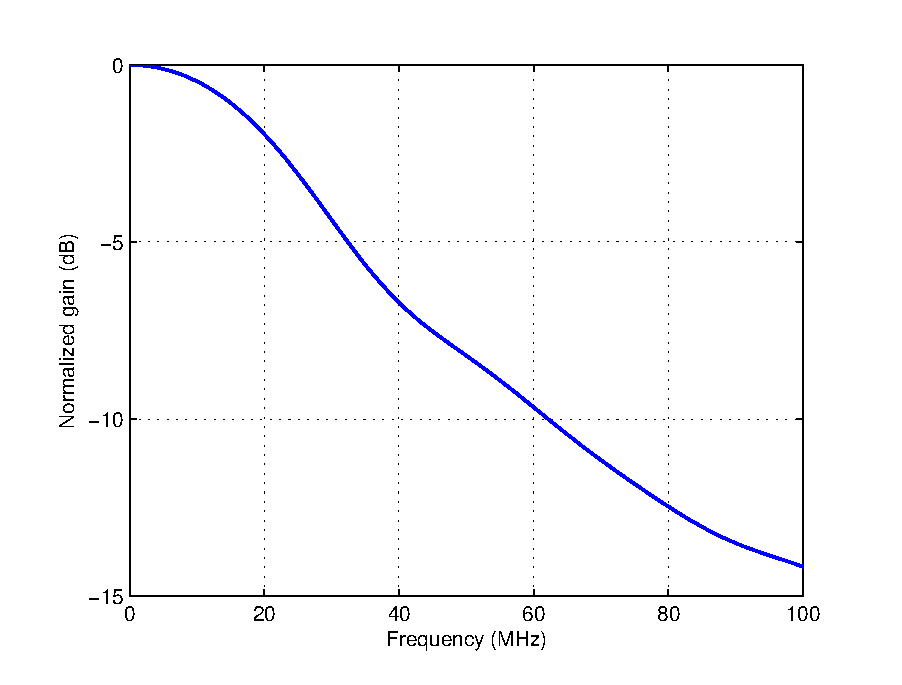
\includegraphics[width=0.5\textwidth]{figures/chapter-3/Sim_Channel_frequency.eps}
    }
    \caption{仿真信道冲激响应}
    \label{fig:ZC_frequency_time}
\end{figure}
仿真主要参数设置如表\ref{tab:Signle Color Channel Estimation Paramters}所示,采用DCO-OFDM调制方式,在每个OFDM帧中放20个OFDM符号,也就是说加上导频,一帧共有21个OFDM符号;从图\ref{fig:Sim_Channel_frequency}中可以看出,可见光信道是一个明显的低通信道,低频端的子载波处信噪比高,可以使用高阶调制,而高频段的子载波上信噪比低,只能使用低阶调制或者设置为虚拟子载波,在仿真中我们设置最低频4个子载波和最高频的4个子载波为虚拟子载波,其他子载波上的调制阶数如表\ref{tab:modOrder}所示。
\begin{table}[ht]
    \caption{信道估计技术仿真参数}
    \label{tab:Signle Color Channel Estimation Paramters}
    \centering
    \begin{tabular}{ll}
        \toprule
        参数名称                & 参数值\\
        \midrule
        信道类型                & 室内可见光信道\\
        多径数量                & 20 \\
        每帧OFDM符号数        & 20 \\
        调制方式                & 256,64,16,4-QAM\\
        光OFDM类型              & DCO-OFDM\\
        FFT长度                 & 256 \\
        可用子载波数            & 128 \\
        低频虚拟子载波          & 4  \\
        高频虚拟子载波          & 4  \\
        循环前缀长度            & 24 \\
        \bottomrule
    \end{tabular}
\end{table}
因为在仿真中使用固定的ZC序列作为导频序列,即公式\ref{equ:MMSE3}中的$\textbf X$为ZC序列张成的对角矩阵,则有:
\begin{equation}
\textbf X \textbf X^H = \textbf I_N;
\end{equation}
所以在这种情况下MMSE估计与LMMSE估计等价,因此在仿真中我们只给出了LMMSE 的结果。

\begin{table}[ht]
    \caption{各子载波上的调制阶数}
    \label{tab:modOrder}
    \centering
    \begin{tabular}{lllll}
        \toprule
        子载波序号    & $4\sim47$  & $48\sim95$  & $96\sim111$ & $112\sim123$ \\
        \midrule
        调制阶数      & 256QAM  & 64QAM  &16QAM & 4QAM    \\
        \bottomrule
    \end{tabular}
\end{table}
图\ref{fig:BER_SNR_avg}展示了在不同信道估计方法下误比特率(Bit Error Rate,BER)随信噪比(SNR)的变化关系,值得注意的是,为了尽量与实际系统吻合,仿真中使用的信噪比是符号信噪比,而不是比特信噪比,并且假设每个子载波上的噪声方差相等。同时,在仿真中计算公式\ref{equ:LMMSE1}和\ref{equ:SVD1}的$\textbf R_{HH}$时,我们取的是从当前帧开始到之前的10帧的信道估计得到的信道自相关矩阵的平均值。可以用下面的公式表示:
\begin{equation}
\textbf R_{HH} = E(\textbf H \textbf H^H)=\frac{1}{10}\sum_{i=0}^{9}\textbf H_i \textbf H_i^H
\end{equation}
其中$\textbf H_i$表示前面第i帧的信道估计。仿真结果表明LS 估计的性能最差,理想信道估计(Ideal)的性能最好,但是这是不可实现的,而LMMSE 估计和SVD 分解法的效果差不多,劣于理想信道估计而优于LS信道估计,LMMSE估计和SVD估计有大约3 dB 的增益,仿真结果与之前的分析吻合。

\begin{figure}[htbp]
\centering
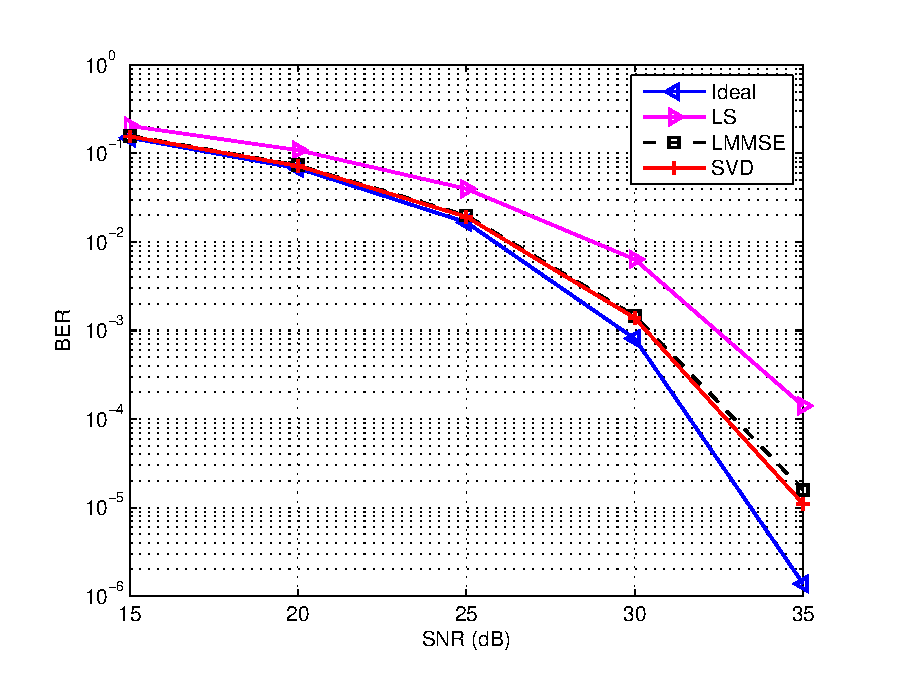
\includegraphics[width=0.8\textwidth]{figures/chapter-3/BER_SNR_avg.eps}
\caption{不同信道估计方法BER性能比较}
\label{fig:BER_SNR_avg}
\end{figure}

\begin{figure}[htbp]
\centering
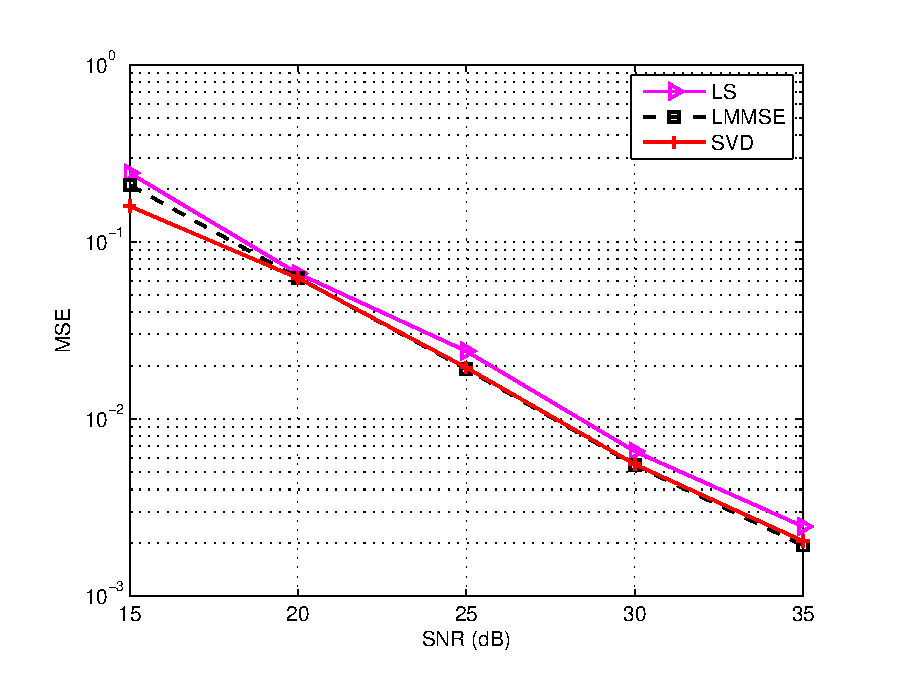
\includegraphics[width=0.8\textwidth]{figures/chapter-3/MSE_SNR_avg.eps}
\caption{不同信道估计方法MSE性能比较}
\label{fig:MSE_SNR_avg}
\end{figure}
图\ref{fig:MSE_SNR_avg}给出了不同信道估计算法的均方误差(Mean Square Error, MSE)性能,均方误差的定义如下:
\begin{equation}
MSE = E\left(\frac{1}{N}\sum_{i=0}^{N-1}|H_R(i)-\hat{H}(i)|^2\right)
\end{equation}
时钟N表示子载波数量,$H_R(i)$表示第i个子载波的真实信道冲激响应,$\hat{H}(i)$表示第i个子载波的信道估计。根据上面的公式,理想信道估计的MSE应该为0,所以在图上我们就没画出了,仿真结果表明LMMSE和SVD信道估计相对于LS信道估计的MSE也有一些提高。

为了进一步比较不同信道估计方法的性能优劣,图\ref{fig:BER_sc}展示了当信噪比设置为25 dB时每个子载波上的BER性能。从图中可以看出,在相同的调制阶数的子载波上,BER 随着子载波序号的增加而升高,这是因为低通信道的作用;在调制阶数变低时,子载波上的BER也剧降。从图中我们也可以看出,这个发射端在子载波上等功率分配的方式使得子载波上的BER方差很大,不利于整体BER性能提高,这方面的分析将在第四章详细说明。
\begin{figure}[htbp]
\centering
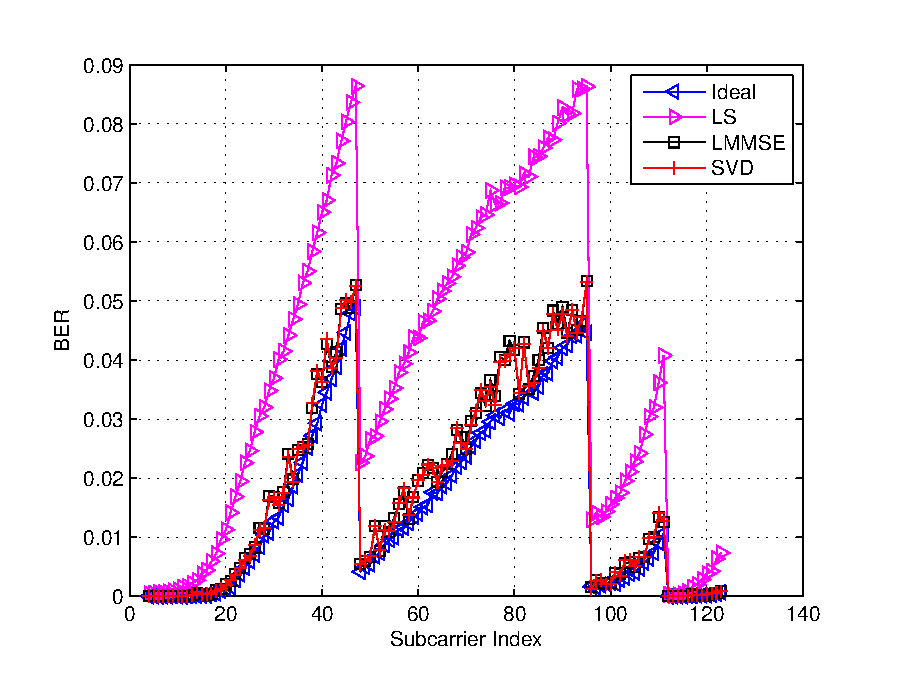
\includegraphics[width=0.8\textwidth]{figures/chapter-3/BER_sc.eps}
\caption{SNR=25 dB时不同子载波上的误比特率}
\label{fig:BER_sc}
\end{figure}


前面在分析基于SVD分解的MMSE算法时提到,为了进一步简化运算,可以只取$\textbf R_{HH}$前$M$个比较大的特征值$\lambda_1,\lambda_2,\cdots,\lambda_M$,将最后N-M 个较小的特征值为零。图\ref{SVD_BER_MSE_SNR_avg}给出了不同M值下BER和MSE性能比较,发现在$M=1$的性能最优,M增大,BER、MSE 性能反而有小许的劣化,当$M=N$时,SVD 与LMMSE 等价(在前面的仿真中选择$M=2$)。
\begin{table}[ht]
    \caption{$\textbf R_{HH}$前10个最大特征值}
    \label{tab:modOrder}
    \centering
    \begin{tabular}{lllllllllll}
        \toprule
        序号 & 1 & 2& 3& 4&5& 6& 7& 8& 9&10 \\
        \midrule
        特征值 &255.865 &1.814&0.032&0.031 & 0.028 & 0.027&0.023&0.021&0.020&0.017\\
        \bottomrule
    \end{tabular}
    \label{tab:tezhengzhi}
\end{table}
为了分析,表\ref{tab:tezhengzhi} 给出了$\textbf R_{HH}$ 最大的10 个特征值,发现第一个值非常大,而后面的都比第一个小很多,这是因为经过SVD 分解之后,最大特征值对应的是主成分,而后面的都是噪声,因此$M=1$时性能最优。这样在使用SVD 进行信道估计时只需使用最大的特征值即可,不仅可以减少一次矩阵减法,而且还有利于提高估计精度。
\begin{figure}[htbp]
    \centering
    \subfloat[不同M值下BER性能比较]{
        \label{fig:Sim_Channel_time}
        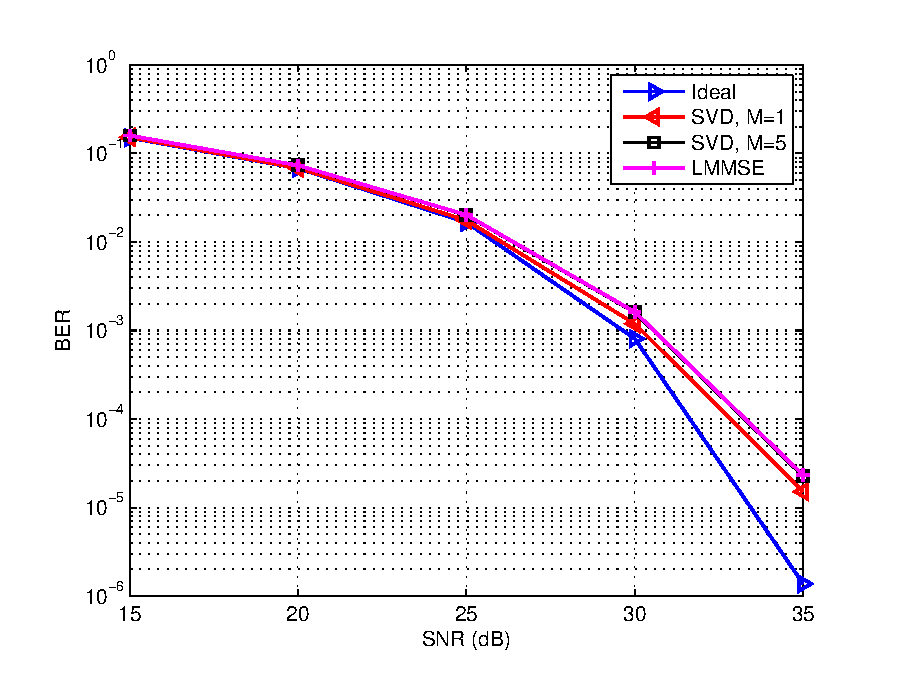
\includegraphics[width=0.5\textwidth]{figures/chapter-3/SVD_BER_SNR_avg.eps}
    }
    \subfloat[不同M值下MSE性能比较]{
        \label{fig:Sim_Channel_frequency}
        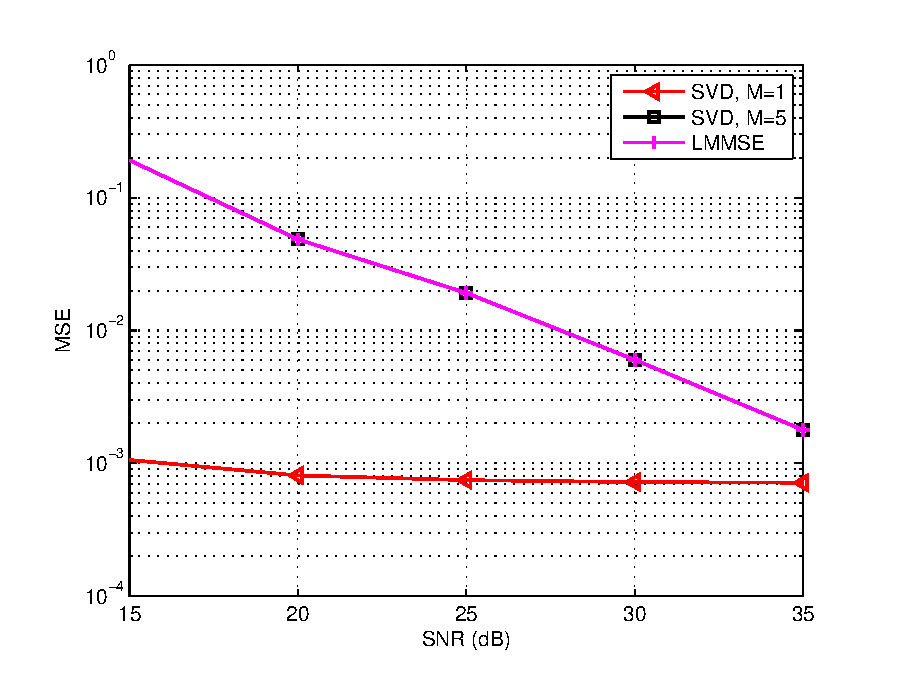
\includegraphics[width=0.5\textwidth]{figures/chapter-3/SVD_MSE_SNR_avg.eps}
    }
    \caption{SVD信道估计方法不同M值下性能比较}
    \label{fig:SVD_BER_MSE_SNR_avg}
\end{figure}
\section{实际系统中的信道估计误差}
进行自适应传输时,不仅需要估计信道的冲激响应以用于解调,还需要估计信道的信噪比信息以选择合适的比特分配和能量分配策略,所以准确的信噪比估计是自适应传输的前提条件。信噪比估计有两种方法,一种是直接使用导频序列,使用式\ref{equ:chapter-3-3},得到信噪比的表达式为:
\begin{equation}
SNR(i) = \frac{|X(i) \hat{H}(i)|^2}{|Y(i)-X(i) \hat{H}(i)|^2}
\end{equation}
其中$SNR(i)$表示第i个子载波处的信噪比,$\hat{H}(i)$表示信道频域响应的估计值,可以是\ref{section:Channel_Estimation}中任意的一种估计方法,$X(i)$表示第i 个子载波上的发射符号,$Y(i)$表示第i个子载波处的接收符号;另一种方法要使用额外的训练序列,称为误差向量幅度法(Error Vector Magnitude,EVM),EVM的定义如下:
\begin{equation}
EVM(i) = |\hat{X}(i)-X(i)|^2
\end{equation}
式中$X(i)$表示第i个子载波上的发射信号,$\hat{X}(i)$表示使用信道估计均衡后的接收信号,EVM与SNR之间的关系是\cite{shafik2006extended}:
\begin{equation}
SNR \approx \frac{1}{EVM^2}
\end{equation}

\begin{figure}[htbp]
\centering
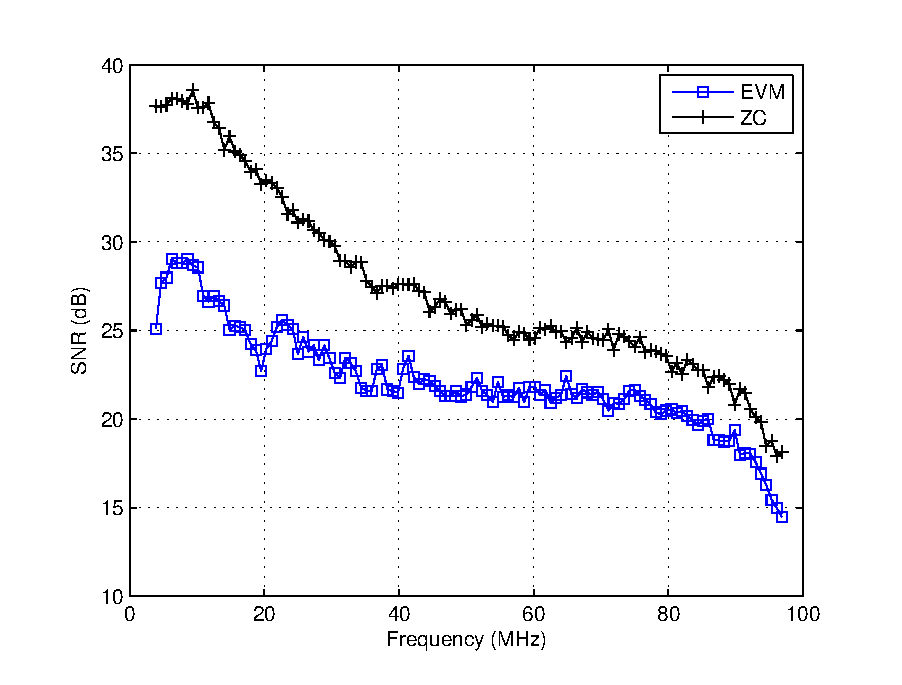
\includegraphics[width=0.8\textwidth]{figures/chapter-3/SNR_ZC_EVM.eps}
\caption{SNR=25 dB时不同子载波上的误比特率}
\label{fig:BER_sc}
\end{figure}
\section{本章小结}
